\documentclass{article}
\usepackage{graphicx}
\usepackage{amsmath}
\usepackage{cite}
\usepackage{float} % Add in the preamble

\title{Technical Report on Simulation Software in Robotics Term Project}
\author{Chengze Song, Bibek Poudel}
\date{\today}

\begin{document}
    \maketitle

    \section{Introduction}
    Our project is the simulation of a rollercoaster-cart over a track. We have considered
    different environmental parameters such as gravity, friction, and air resistance.
    The goal is to simulate the motion of the cart over the track and to analyze
    the forces acting on the cart. Our roller coaster simulation model is felxible
    for the user/designers as they can tweak all the parameters to test different
    real world scenarios. We have used Matlab/Simulink, Python, and solidworks
    for the project. The simulation results and project details are discussed in
    the following sections.

    \section{Problem Statement}
    This project aims to simulate the motion of a rollercoaster-cart over a track.
    The cart is subject to gravity, friction, and air resistance. The cart is subjected
    to a initial thrust by a PMLSM motor which provides thrust for 4 sec over a horizontal
    track. The goal is to analyze the forces acting on the cart and to simulate
    the motion of the cart over the track. The track is composed of different sections
    with varying slopes(Horizontal, and Inclined). The simulation results will
    be used to analyze the forces acting on the cart and determine whether the
    thrust provided by the motor is sufficient to move the cart over the track.
    \subsection{System and Environment}
    % Clearly state the problem statement, indicate the system and its environment.
    Our system of interest is a rollercoaster-cart moving over a track. Our
    environment includes gravity, friction, roller-coaster track and air
    resistance

    \subsection{Desired Inputs and Outputs}
    \textbf{\textit{First Subsystem(PMLSM Motor):}}
    \newline
    \textbf{\textit{Inputs:}}
    \begin{itemize}
        \item The desired behaviour of the position of the rollercoaster

        \item The parameters of the motor For example:
            \begin{itemize}
                \item $F_{\text{max}}$: 2000 N (Maximum thrust generated by the motor).

                \item $PM$: 0.65 Wb (Permanent magnet flux linkage).

                \item $L_{d}$: 0.01 H (Inductance along the d-axis).

                \item $L_{q}$: 0.01 H (Inductance along the q-axis).

                \item $L_{0}$: $2 \times 10^{-4}\, \text{H}$ (Zero-sequence axis
                    inductance).

                \item $R_{s}$: 0.6 ohm (Stator resistance).

                \item Mass: 1000 kg (Mass of the moving part).

                \item Pitch: 0.1 m (Polar pitch or distance between poles).

                \item $N_{p}$: $\pi/\text{Pitch}\, \text{rad/m}$ (Electrical pole-pair
                    constant).
            \end{itemize}
    \end{itemize}

    \textbf{\textit{Outputs:}}
    \begin{itemize}
        \item Thrust provided by the motor
    \end{itemize}
    \textbf{\textit{Second Subsystem(Roller Coaster):}}
    \newline
    \textbf{\textit{Inputs:}}
    \begin{itemize}
        \item Track Profile i.e the length of the track and slope of the track

        \item Environmental parameters such as gravity, friction, and air resistance

        \item The thrust provided by the motor
    \end{itemize}
    \textbf{\textit{Outputs:}} \begin{itemize} \item Motion of the cart over the
    track \item Forces acting on the cart (gravitational force, frictional force,
    air resistance) \item Analysis of whether the thrust provided by the motor is
    sufficient to move the cart over the track \item Acceleraton, velocity, and position
    of the cart at each time step which is then provided as a feedback to solve the
    ordinary differential equations to get the next state of the system.

    \section{Relevance in Mechatronics and Robotics}
    % Cite at least one journal paper to indicate how this problem is relevant in the field of mechatronics and robotics.
    Often Engineering design projects are tested using simulation software before
    the actual implementation. Engineering projects are complex, costly and margin
    of error is very low. Simulation software helps to test the design and
    analyze the performance of the system before the actual implementation. The simulation
    of the rollercoaster-cart over a track is relevant in the field of mechatronics
    and robotics as it helps to analyze the forces acting on the cart and determine
    whether the thrust provided by the motor is suhe cart over the track . The simulation
    results can be used to optimize the design of the rollercoaster-cart and to analyze
    the performance of the system. Furthermore, based on the simulation results,
    different parameters such as the g forces experienced by the cart, the maximum
    speed of the cart, and the energy consumption of the motor can be analyzed
    which can be used to optimize the design of the rollercoaster-cart. Over the
    years mechanical dynamics has been a part of mechatronics and robotics curriculum.
    Due to advancement in computing power, simulation software has become an integral
    part of the design process of dynamical systems. The simulation of the
    rollercoaster-cart over a track is a good example of how simulation software
    can be used to analyze the performance of a dynamical system and to optimize
    the design of the system. Simulation softwares can be used to model different
    design parameters for consideration and get the best possible design for the
    system without using any physical resources,which is cost-effective and time-saving.\textsuperscript{1}

    \section{Models Used}
    \subsection{Diagrams and Equations}
    % Describe the models used, use diagrams and/or equations as appropriate.
    The model of the rollercoaster-cart over a track is based on the following equations:
    The model of the rollercoaster-cart over a track is based on the following
    equations:
    \begin{equation}
        F_{\text{net}}= m \cdot a
    \end{equation}
    \begin{equation}
        F_{\text{net}}= F_{\text{thrust}}- F_{\text{gravity}}- F_{\text{friction}}
        - F_{\text{air resistance}}
    \end{equation}
    \begin{equation}
        acceleration = \frac{dv}{dt}
    \end{equation}
    The initial condition of the velocity integration is the final velocity of the
    part where the thrust is provided
    \begin{equation}
        velocity = \frac{dx}{dt}
    \end{equation}
    \begin{equation}
        F_{\text{gravity}}= m \cdot g \cdot \sin(\theta)
    \end{equation}
    \begin{equation}
        F_{\text{friction}}= m \cdot g \cdot \cos(\theta)
    \end{equation}
    \begin{equation}
        F_{\text{air resistance}}= 0.5 \times \rho \times A \times C_{d} \times v
        ^{2}
    \end{equation}
    \begin{figure}[H]
        \centering
        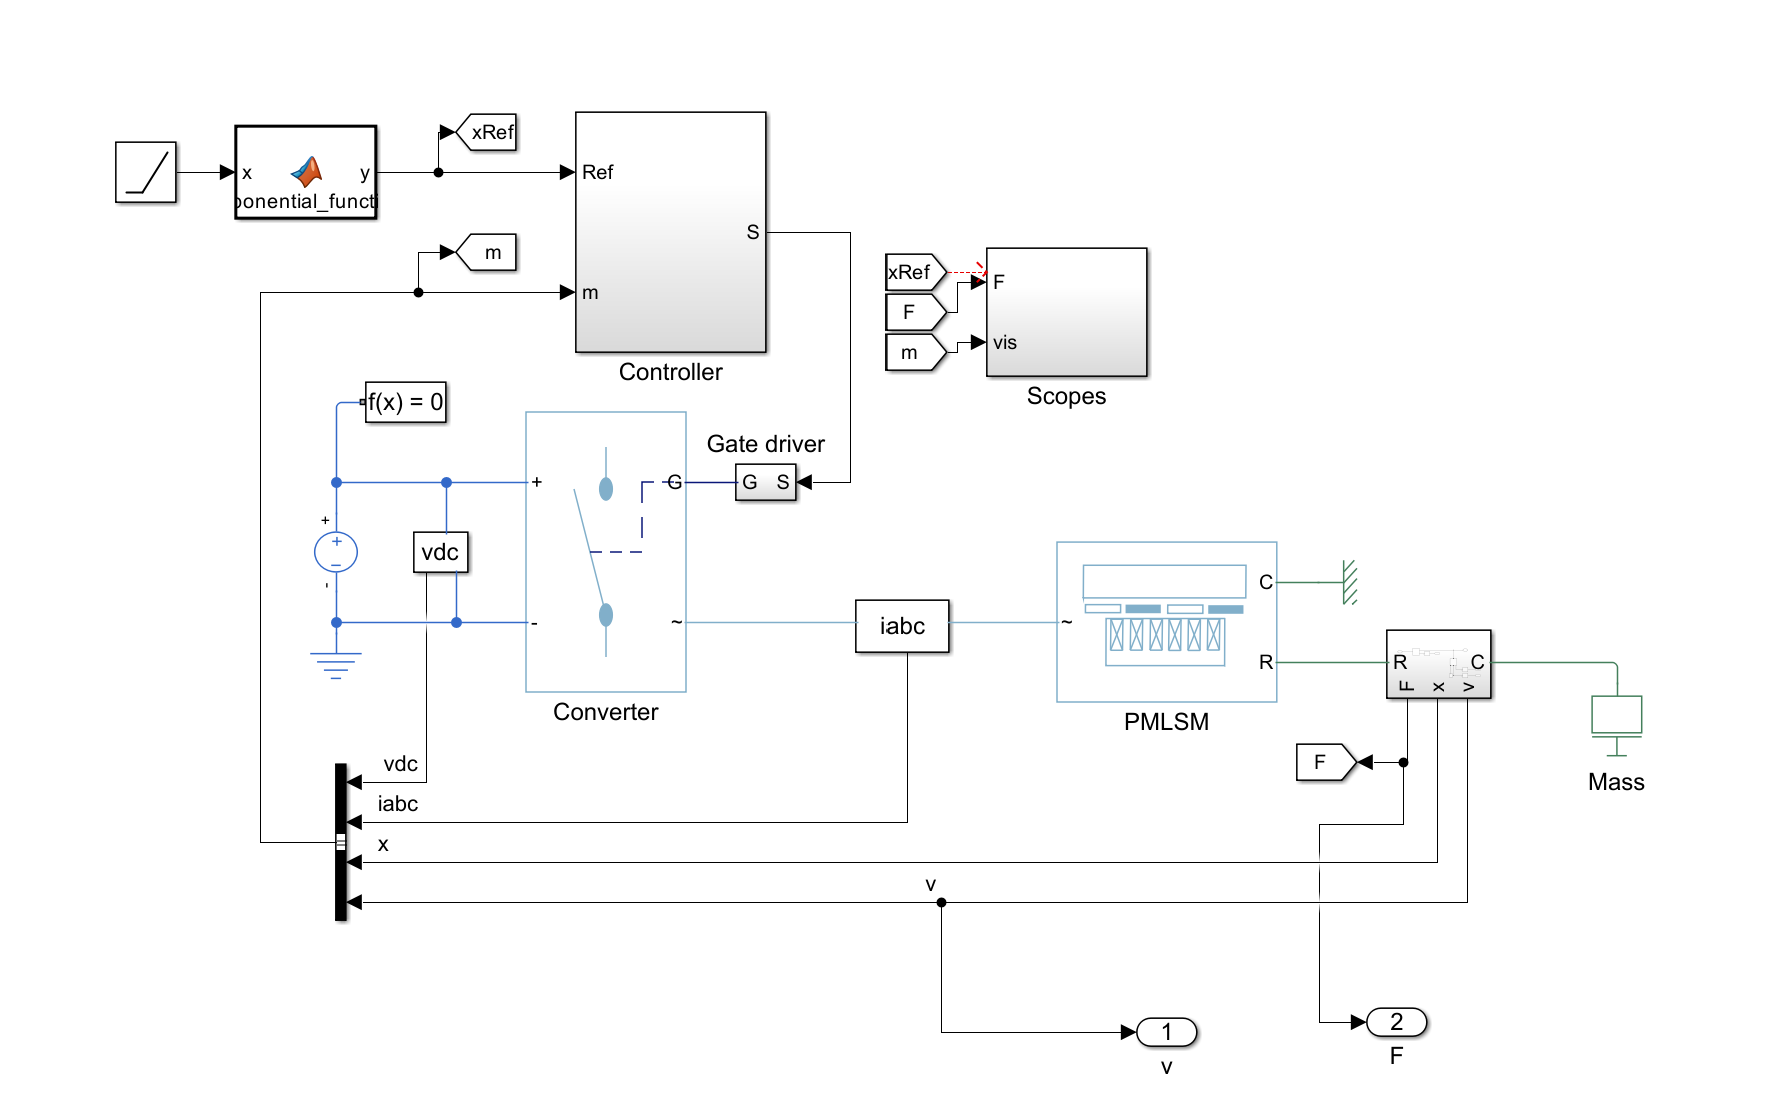
\includegraphics[width=0.9\textwidth]{
            ./Snapshots/Screenshot 2024-12-08 042938.png
        } % Corrected the path
        \caption{Motor Model}
        \label{fig:Motor Model}
    \end{figure}
    \textbf{Motor Model:} This diagram demonstrates position control in a three-phase
    Permanent Magnet Linear Synchronous Machine (PMLSM) drive using a PI-based
    cascade control structure. The control system includes an outer position loop,
    a speed loop, and two inner current loops. The PMLSM is powered by a
    controlled three-phase converter, with step references guiding the simulation.
    Results are visualized using the Scopes subsystem.

    \begin{figure}[H]
        \centering
        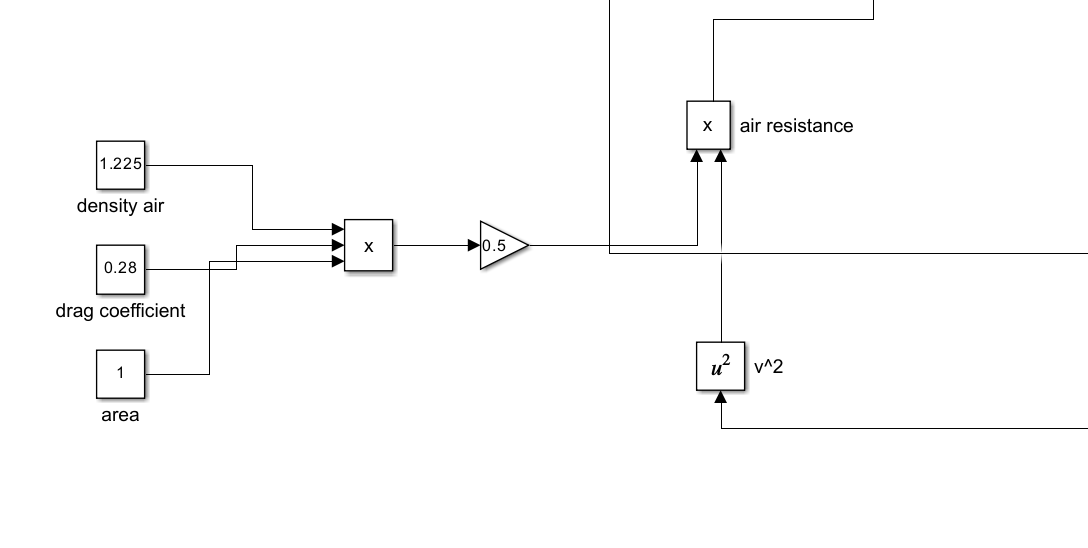
\includegraphics[width=0.7\textwidth]{
            ./Snapshots/air_resistance.png
        } % Corrected the path
        \caption{Air resistance model}
        \label{fig:Air resistance model}
    \end{figure}
    \textbf{Air Resistance Model:} This diagram demonstrates the air resistance model.
    The air resistance is modelled as a function of the velocity of the cart. The
    air resistance is calculated using the formula $F_{\text{air resistance}}= 0.
    5 \times \rho \times A \times C_{d} \times v^{2}$ where $\rho$ is the air density,
    $A$ is the cross-sectional area of the cart, $C_{d}$ is the drag coefficient,
    and $v$ is the velocity of the cart.
    \begin{figure}[H]
        \centering
        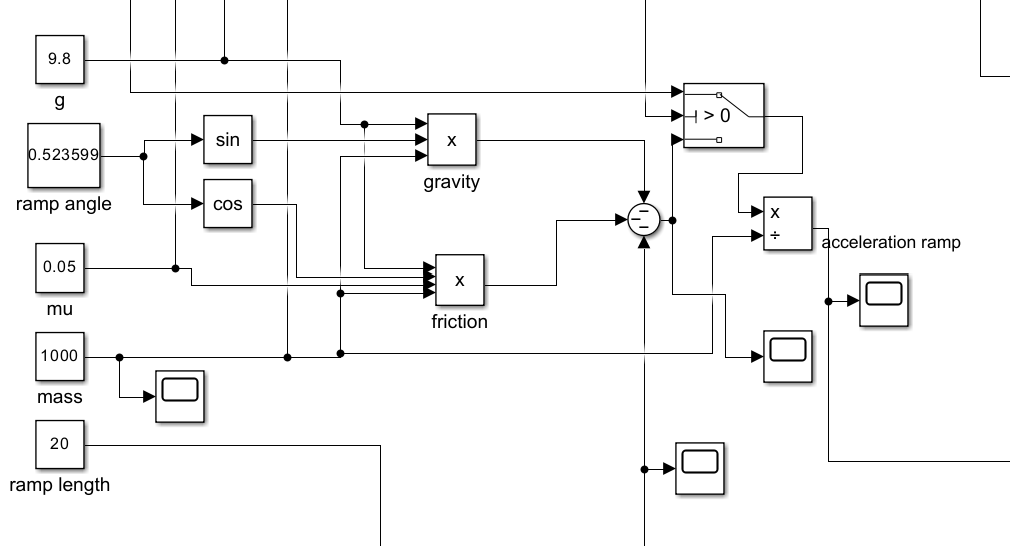
\includegraphics[width=0.7\textwidth]{
            ./Snapshots/friction_gravity.png
        } % Corrected the path
        \caption{Friction and Gravity model}
        \label{fig:Friction and Gravity model}
    \end{figure}
    \textbf{Friction and Gravity Model:} This diagram demonstrates the friction
    and gravity model. The friction and gravity are modelled as a function of the
    angle of the track. The friction is calculated using the formula
    $F_{\text{friction}}= m \cdot g \cdot \cos(\theta)$ and the gravity is
    calculated using the formula
    $F_{\text{gravity}}= m \cdot g \cdot \sin(\theta)$ where $m$ is the mass of
    the cart. $g$ is the acceleration due to gravity, and $\theta$ is the angle
    of the track.
    \begin{figure}[H]
        \centering
        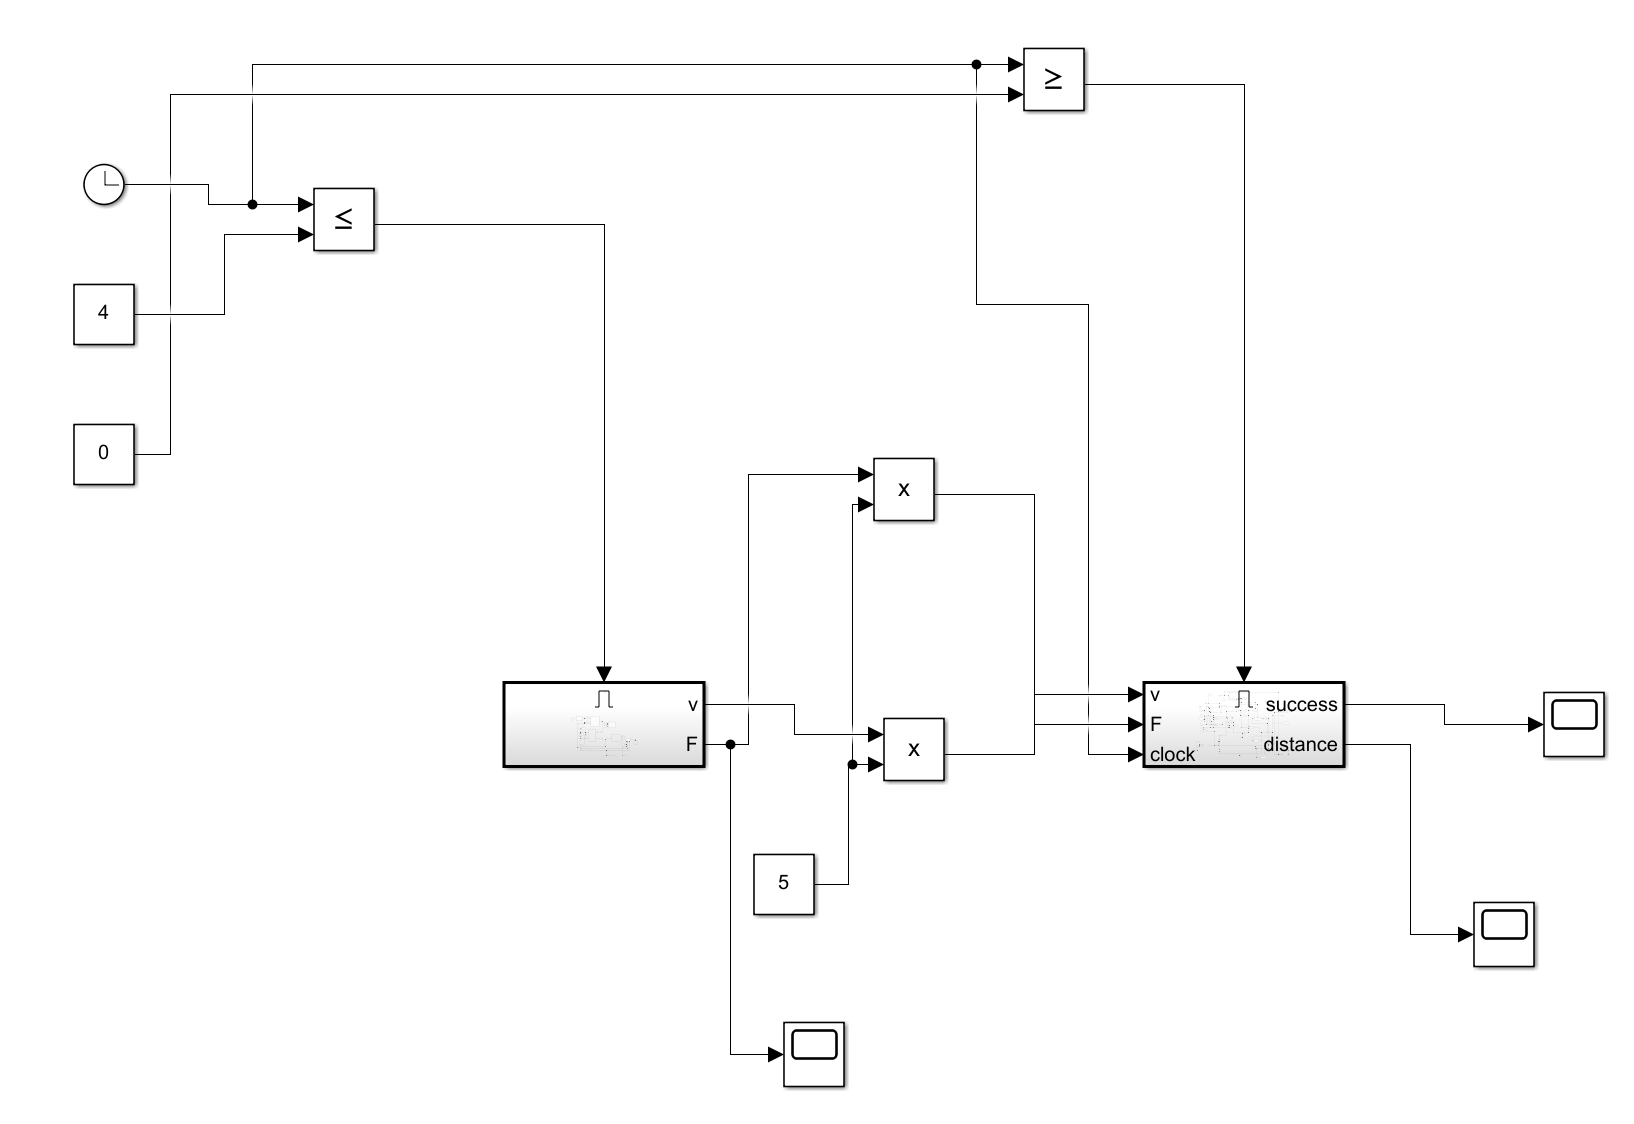
\includegraphics[width=0.9\textwidth]{
            ./Snapshots/system_integration.png
        } % Corrected the path
        \caption{System Integration}
        \label{fig:System Integration}
    \end{figure}
    \textbf{System Integration:} This diagram demonstrates the integration of
    the PMLSM motor and the rollercoaster model.
    \begin{figure}[H]
        \centering
        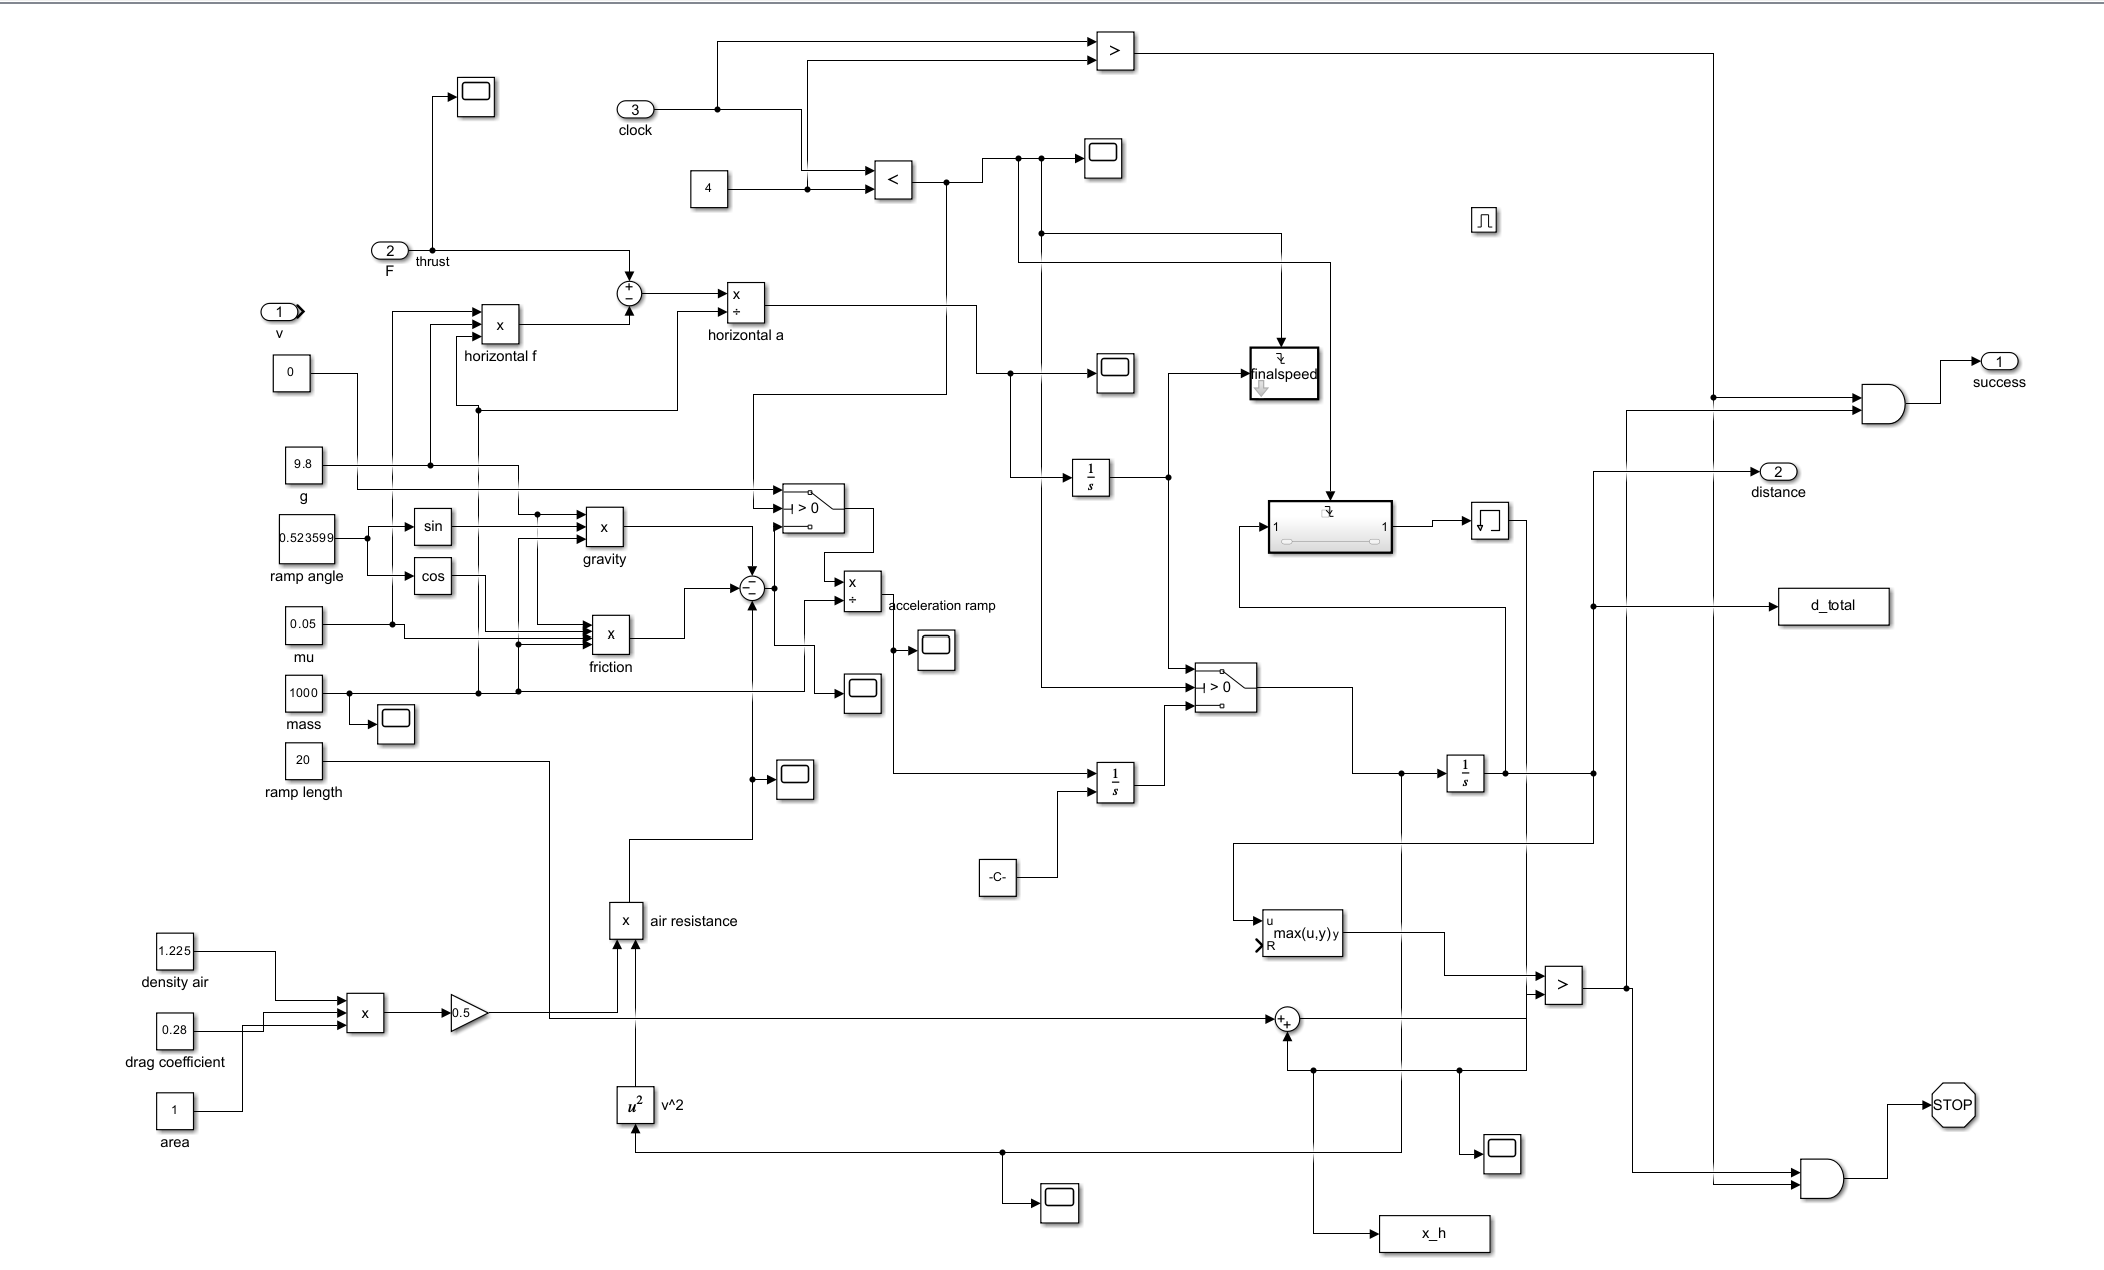
\includegraphics[width=1\textwidth]{
            ./Snapshots/Main_Block.png
        } % Corrected the path
        \caption{Roller Coaster System}
        \label{fig:Roller Coaster System}
    \end{figure}
    \textbf{Roller Coaster System:} This diagram demonstrates the rollercoaster
    system. The rollercoaster system includes the thrust from the PMLSM motor,
    the rollercoaster model, and the environmental parameters such as gravity,
    friction, and air resistance. A switch block is used to provide thrust to
    the cart for specific time over a horizontal track. Then the cart moves over
    an inclined track.

    \subsection{System Parameters and State Variables}
    % Identify the system parameters and the state variables.
    % ...existing code...\idotsint

    \subsection{Assumptions and Justifications}
    % Identify any assumptions in the model and how they are justified.
    % ...existing code...
    \begin{enumerate}
        \item There is no air resistance in the horizontal section of the track :
            The linear synchonous motor uses feedback control system to provide thrust
            to the cart. Due to the feedback control system, the thrust compensates
            for the air resistance in the horizontal section of the track.

        \item Friction is constant throughout the track: The track is made of
            same material throughout the track. The coeffiecient of friction is constant
            throughout the track as the track is made of same material.

        \item Due to the problem of the integration, we are not considering the
            sharp incline of the track.

        \item The PI controllers have idealized behavior with no delay or non-linearities.
            This assumption simplifies initial control design and tuning. Any real-world
            imperfections can be addressed later during implementation.

        \item The cart is assumed to be a point mass: The cart is assumed to be
            a point mass to simplify the analysis. The mass of the cart is concentrated
            at the center of mass of the cart

        \item Mechanical losses such as friction, windage, and eddy currents are
            ignored or minimally considered.These effects are small compared to the
            overall system dynamics and can be incorporated later if needed.
    \end{enumerate}

    \subsection{Code Documentation}
    % Provide documentation on how to use the code including but not limited to settings and relevant explanations of why certain functions were used.
    % ...existing code...
    % numeric bulletin and italicized steps
    \begin{enumerate}
        \item \textit{Open the Matlab/Simulink model file:} The Matlab/Simulink
            model file contains the simulation of the rollercoaster-cart over a
            track. The model file contains the block diagram of the system and the
            parameters of the system.

        \item \textit{Run the simulation:} Run the simulation to simulate the
            motion of the cart over the track. The simulation results will be displayed
            in the scope block.

        \item \textit{Use scope to analyze:} Use the scope block to analyze the
            motion of the cart over the track. Based on the requirements there are
            different scopes. The scope block can be used to analyze the forces
            acting on the cart and to determine whether the thrust provided by
            the motor is sufficient to move the cart over the track, position,
            velocity, air resistance e.t.c.

        \item \textit{Change the parameters in simulation:} The parameters of
            the system such as the initial thrust provided by the motor, the track
            profile, and the environmental parameters can be changed in the
            simulation to analyze the performance of the system under different
            conditions.
    \end{enumerate}

    \section{Computational Results and Discussion}
    \subsection{Results}
    % Show computational results and adequate discussion of those results, use figures as appropriate.
    % ...existing code...
    The simulation results of the rollercoaster-cart over a track are shown in the following figures:
    \begin{enumerate}
        \item \textbf{Scenario 1 :}\newline \textbf{When the thrust provided by the motor is insufficient to move the cart}
        \newline
        Expected Result: The cart will move along the track but will not reach the top of the ramp. At a certain point the cart will stop and move in opposite direction.
        \item \textbf{Scenario 2 :}\newline \textbf{When the thrust provided by the motor is sufficient to move the cart}
        \newline
        Expected Result: The cart will move along the track and reach the top of the ramp. The cart will move along the track and reach the end of the track.
        \item 
    \end{enumerate}


    \section{Validation}
    % Show some form of validation of your simulation results.
    % ...existing code...
    The validation of the simulation results is performed using the \textbf{principle
    of conservation of energy}, which states that the total energy in a system remains
    constant unless acted upon by an external force. For the rollercoaster-cart
    system, the total mechanical energy is the sum of \textit{kinetic energy (KE)},
    \textit{potential energy (PE)}, and the work done against friction and air resistance.

    The key equations are:

    \begin{enumerate}
        \item \textbf{Kinetic Energy (KE):}
            \begin{equation}
                KE = \frac{1}{2}m v^{2}
            \end{equation}
            where $m$ is the mass of the cart and $v$ is its velocity.

        \item \textbf{Potential Energy (PE):}
            \begin{equation}
                PE = m g h
            \end{equation}
            where $g$ is the gravitational acceleration, and $h$ is the height relative
            to a reference point.

        \item \textbf{Work done against friction and air resistance:}
            \begin{equation}
                W_{\text{loss}}= F_{\text{friction}}\cdot d + F_{\text{air
                resistance}}\cdot d
            \end{equation}
            where $F_{\text{friction}}$ and $F_{\text{air resistance}}$ are the
            forces due to friction and air resistance, respectively, and $d$ is
            the distance traveled.
    \end{enumerate}

    Using these equations, we validate the simulation by ensuring that:
    \begin{equation}
        \text{Total Energy Input}= KE + PE + W_{\text{loss}}
    \end{equation}

    \subsection{Validation Procedure}

    \begin{enumerate}
        \item \textbf{Initial State:} At the start of the simulation, the cart has
            an initial thrust energy imparted by the PMLSM motor. This energy is
            calculated as the work done by the motor over the time it is active:
            \begin{equation}
                E_{\text{motor}}= F_{\text{thrust}}\cdot d_{\text{thrust}}
            \end{equation}

        \item \textbf{Energy Transitions:} As the cart moves, the thrust energy is
            converted into kinetic energy, potential energy (on inclined tracks),
            and energy lost due to friction and air resistance. At every time
            step, the simulation tracks these components.

        \item \textbf{Validation Check:} At several points along the track, the total
            energy calculated from the simulation results is compared with the expected
            energy from the conservation of energy equation. Deviations are
            checked for numerical errors or unaccounted forces.
    \end{enumerate}

    \subsection{Observations}
    \begin{itemize}
        \item On horizontal sections of the track, the change in kinetic energy
            corresponds closely with the work done by the thrust, friction, and
            air resistance.

        \item On inclined sections, the increase in potential energy matches the
            reduction in kinetic energy and the work done against gravity.

        \item The overall energy balance is maintained within acceptable tolerances,
            confirming the simulation's accuracy.
    \end{itemize}

    This validation demonstrates that the simulation adheres to fundamental
    physical laws, providing confidence in its results.

    \section{Discussion}
    % Discuss the advantages and disadvantages of the simulation platform you chose for this problem.
    % If results do not agree with expectations, offer possible explanations why and demonstrate the knowledge gained.
    % Mention the limitations of your work.
    % ...existing code...
    Advantages and Disadvantages of Matlab/Simulink:
    \begin{enumerate}
        \item Advantages:
            \begin{enumerate}
                \item Matlab/Simulink is widely used in the industry for modeling
                    and simulation of dynamical systems. The software is used in
                    various fields such as control systems, robotics, and
                    mechatronics.

                \item The software provides a graphical user interface for modeling
                    and simulation of dynamical systems. The user can drag and
                    drop blocks to model the system and simulate the system.

                \item The software provides a wide range of blocks for modeling different
                    components of the system such as sensors, actuators, controllers,
                    and plant models.

                \item The software provides a wide range of solvers for simulating
                    the system. The user can choose the appropriate solver based
                    on the dynamics of the system.

                \item The software provides a wide range of training options for
                    learning how to use the software. The user can take online
                    courses, attend workshops, and get certified in using the
                    software.
            \end{enumerate}

        \item Disadvantages:
            \begin{enumerate}
                \item The learning curve of Simulink is steep. It takes time to
                    learn how to use the software effectively. The user needs to
                    have a good understanding of the system dynamics and control
                    theory to model the system accurately.

                \item The software is expensive. The user needs to purchase a
                    license to use the software. The cost of the software can be
                    a barrier for small companies and individuals.

                \item The software is not open-source. The user cannot modify
                    the source code of the software. The user is limited to the features
                    provided by the software.

                \item The software is not platform-independent.
            \end{enumerate}
    \end{enumerate}

    \subsection{Limitations}
    % Discuss the limitations of your work.
    % ...existing code...
    The limitations of the simulation of the rollercoaster-cart over a track :
    \begin{enumerate}
        \item The simulation does not consider the effect of environmental factors
            such as temperature, humidity e.t.c. These factors can affect the friction.

        \item The simulation does not consider the effect of vibrations on the cart.
            Vibrations can affect the motion of the cart over the track.

        \item The simulation does not consider the whole rollercoaster track. It
            only considers a small section of the track. The simulation can be extended
            to consider the whole track.
    \end{enumerate}
    \section{Conclusion}
    % ...existing code...
    In conclusion, the simulation of the rollercoaster-cart over a track has
    been successfully implemented using Matlab/Simulink, Python, and solidworks.
    The simulation results have been used to analyze the forces acting on the cart
    and to determine whether the thrust provided by the motor is sufficient to move
    the cart over the track. The simulation results coincides with the
    expectations. The results obtained from the simulation can be used as a reference
    for the development of the rollercoaster system in the real world. With the
    developement of computing power, we can simulate more complex systems and analyze
    the perfermance of the system before the actual implementation.

    \section{References}
    % Any sources of information used should be clearly cited within the text and in a bibliography.
    %bullet numbering
    \begin{enumerate}
        \item Teng, Rumin, et al. “Dynamic Modeling and Simulation of Roller
            Coaster.” IEEE Xplore, 2010, ieeexplore.ieee.org/abstract/document/5620012.
            Accessed 21 Apr. 2021.
    \end{enumerate}
\end{document}